\chapter{Introduction}
\label{chap1}
\noindent This project is totally dedicated to the Network Engineer for new and smart learning of the Network Structure. In this concept it is possible for the networker to check the Network Structure of a company spread in the big campus area. The incoming and the outgoing traffic can be maintained along with some security concepts as well. In this logic we use the multiple Routing Protocols in different areas of the university. The practical shows us the proper movement of the packet from one part of the company to the other part of the company. The project comprises of the different departments spread in different buildings of the company. Multiple Routing protocols have been used in different branches and all the departments can communicate with other different departments through the Redistribution among different Routing Protocols.\\

\noindent The East Building has a DHCP server for assigning the IP Addresses to the Hosts in the building as well as a DHCP server has been used in the West Building as well. The Internet Service Provider has been used for Communication of the East and West Building with the Data Centre and Internet through ISP, using the Frame Relay Switching Technology available for Wide Area Network. Routing Protocols EIGRP along with the Synchronous Number, Static Routing, and its concepts including the Default Routing as well has been applied. The different Routing Protocols are running and which has been synchronized to work with Frame Relay Switching Technology.

\section{Objectives}
%
%
The objectives of this project are:
%
%for 1,2,3 numbers
\begin{enumerate}
\item To get familiar with how to established a network for any company. 
%
\item To simulate the network using Cisco Packet Tracer.
%
\item To get familiar with networking protocols.
%
%
\end{enumerate}
\section{Introduction}
Technology has reached its highest peak of development, especially in making
life easier for people. Well implemented technology is faster than human in processing
calculation and is more accurate. Technology has become an important concept in our
life. It assists in connecting communities together. Obviously, people have started to use
technology in every field of life including education, health, the military, etc.
The computer network represents a component, especially on how it enhances the
functional performance in different fields and organizations, such as companies and
schools.\\

A school�s computer network performs so many functions, such as connecting
students with the university, faculty, and the library. Most universities today use the
network to provide online education by connecting widely dispersed students with their
professors directly.
\begin{figure}[H]  %h=positioning
\begin{center}
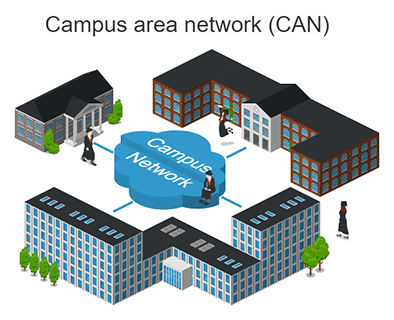
\includegraphics[scale=0.60]{Chapter1/campusNetwork}
\caption{A Campus Network}
\label{figure1}
\end{center}
\end{figure}
\noindent For this reason, computer networks play a vital role in the education
area by providing efficient communications for the university environment.
However, the design of computer networks differs from one university to another.
This is as a result of many factors which determine the differences. Such factors include;
adaptability, integration, resilience, security, and cost. Installing networks in a university
relies on the university�s budget, which differs by institution and from country to country.\\

For instance, there are many countries whose universities do not have the financial
capability for designing the �perfect� or ideal network. Yet these universities from these
third world countries still need to have good quality and more secure network equipment
with less cost. This is because these schools aspire to deliver capability in line with the
leading prestigious universities despite low budgets. 

\section{Motivation}
The word �digital� is very significant in today�s world, with an increase in the development of technology the entire world is moving towards the digital era. The educational institution plays an important role in this digitalization, hence the campus should adapt to digital means of networking as well and become a �digital campus�.\\

Campus networking becomes an important part of campus life and provides the main way for teachers and students to access educational resources, which gives an important platform to exchange information. As laptops and intelligent terminals are widely used, demand for access to information anytime and anywhere has become more and more urgent. Campus network provides an efficient way to explore the internet with a mobile terminal for teachers and students. This is an important mark of the modern campus. With the development of network and communication technology, cable networks on a university campus bring much convenience for teaching and research work.

%Motivated by the emergence of technological advancements and challenges in ...


%
%

%
%\section{UN Stainability Goals}

 %Goal 8 is shown which is Promote sustained, inclusive and sustainable economic growth, full and productive employment and decent work for all. As we will also discuss the economical long time benefits in next chapters. Our project will help industry in economic growth as well as it is providing a help to the meter readers.



%The conceptual frame work for the proposed method is comprises of three basic building blocks and detailed model is shown in Fig. \ref{fw}.
%\begin{enumerate}
%\item Network Formation Block.
%\item Neighbourhood Based Network Matrix Formation Block.
%\item Consensus Formation Block.
%\end{enumerate}
%
%In the network formation block, ...
%
%\FloatBarrier
%\begin{figure}[H]
%\begin{center}
%\hspace{15mm}
%\includegraphics[scale=0.35]{Chapter1/robocanesinternalstates}
%
%\protect\caption{Pseudo-code of Proposed Scheme for Cooperative Control of Networked Multi-Agent Systems.}
%\label{scode}
%\end{center}
%\end{figure}
%
%
\section{Report Break Down}
%
%This thesis deals with convergence analysis .... The main contributions of this work are summarized as follows:
%
%\begin{enumerate}
%\item  Initially a design ....
%
%\item An extended ....
%
%
%\item Modeled a ....
%
%\end{enumerate}
%
%The main contribution of this work is to propose a new way ....
%
%
%
%
%\section{Thesis Outline}
%
%
The major focus of this report is on the findings of the proposed project i.e. University Network using Cisco Packet Tracer.

This Report is organized as follows:
\vspace{5mm}

In chapter 2, literature review is provided in detail about the work which is already been done on Network using Cisco Packet Tracer and will give a brief details about the articles, papers and literature review.
\vspace{5mm}


In Chapter 3, Proposed Methodology is presented in which you will be able to see the method we will work on the designing of a complete project source code to the diagrams.

\vspace{5mm}


In Chapter 4, Result and Simulations are being discussed, in which you will see all kind of finding related to the Campus Network using Cisco Packet Tracer.

\vspace{5mm}

In Chapter 5, we have concluded and summarized the project work and also presented few new research ideas for future studies.


%\begin{equation}
%F=\sum_{n=0}^i(x_i(0)-x_j(0))^2
%%stackrel[u]{v}{T}=\stackrel[u]{v}{L}+\stackrel[u]{v}{L}\underset{W\epsilon V\cap w\neq u}{\sum}\stackrel[v]{w}{L}
%\end{equation}
